\documentclass[12pt]{article}

\usepackage[margin=3cm]{geometry}
\usepackage{amsmath, amssymb, amsthm}
\usepackage{tikz}
\usetikzlibrary{positioning}
\usepackage{tasks}
\usepackage[inline]{enumitem}
\usepackage{tcolorbox}
\tcbuselibrary{breakable}
\usepackage{fancyhdr}

% Initialize line spacing to 1.5
\linespread{1.5}

% LCM and GCF operators
\DeclareMathOperator{\lcm}{lcm}
\DeclareMathOperator{\gcf}{gcf}

% Simple exercises environment using basic enumerate
\newcounter{exercisenum}
\newenvironment{exercises}{%
  \begin{tcolorbox}[colback=white,colframe=black,arc=0pt,breakable]
%   \noindent\textbf{Exercises}\par
  \begin{enumerate}[label=\arabic*),leftmargin=1cm,resume=exercises]
  \setcounter{enumi}{\value{exercisenum}}
}{%
  \setcounter{exercisenum}{\value{enumi}}
  \end{enumerate}
  \end{tcolorbox}
}

% Setup footer for first page only
\fancypagestyle{firstpage}{
  \fancyhf{}
  \fancyfoot[L]{\small FACTORS}
  \fancyfoot[R]{\small \quad Ewan Short \quad \today}
  \fancyfoot[C]{\small\thepage}
  \renewcommand{\headrulewidth}{0pt}
  \renewcommand{\footrulewidth}{0pt}
}

\begin{document}

\thispagestyle{firstpage}

\section{Factors}
\begin{itemize}
\item
\underbar{Division} splits a number into equal parts, or finds how many times one number fits into another.
\item
A \underbar{factor} of a whole number is another whole number that divides it without remainder. We can find all a number's factors by dividing by $1, 2, 3,\ldots$, stopping when we find a factor we already have. For example, to find the factors of 24,
$$
\begin{array}{lc}
24 \div 1 = 24, & \text{$24$ and $1$ are factors,} \\
24 \div 2 = 12, & \text{$12$ and $2$ are factors,} \\
24\div 3 = 8, & \text{$8$ and $3$ are factors,} \\
24\div 4 = 6, & \text{$6$ and $4$ are factors,} \\
24\div 5 = 4+\frac{4}{5}, & \text{$5$ is not a factor,} \\
24\div 6 = 4, & \text{$4$ and $6$ are factors. Stop!} \\
\end{array} 
$$
So the factors of 24 are 24, 1, 12, 2, 8, 3, 6, and 4.
\end{itemize}

\begin{exercises}
\item
Fill in the missing numbers to find all the factors of 6.
$$
\begin{array}{lc}
6 \div 1 = 6, & \text{$6$ and $1$ are factors,} \\
6 \div 2 = \boxed{\phantom{3}}, & \text{$\boxed{\phantom{3}}$ and $2$ are factors,} \\
6 \div 3 = \boxed{\phantom{2}}, & \text{$\boxed{\phantom{2}}$ and $3$ are factors. Stop!} \\
\end{array} 
$$
So the factors of 6 are 6, 1, \boxed{\phantom{3}} and 2. \label{Ex:factors_6}
\item
Find all the factors of 8.
\end{exercises}

\begin{itemize}
\item
A \underbar{common factor} of two numbers is a factor of both. Let's find the common factors of 4 and 8. First, find all the factors of 4.
$$
\begin{array}{lc}
4 \div 1 = 4, & \text{$4$ and $1$ are factors,} \\
4 \div 2 = 2, & \text{$2$ and $2$ are factors. Stop!} \\
\end{array} 
$$
So the factors of 4 are 1, 2, and 4. Now find all the factors of 8.
$$
\begin{array}{lc}
8 \div 1 = 8, & \text{$8$ and $1$ are factors,} \\
8 \div 2 = 4, & \text{$4$ and $2$ are factors,} \\
8 \div 3 = 1+\frac{3}{8}, & \text{$3$ is not a factor,} \\
8 \div 4 = 2, & \text{$2$ and $4$ are factors. Stop!} \\
\end{array} 
$$
So the factors of 8 are 1, 2, 4, and 8. Thus the common factors of 4 and 8 are 1, 2, and 4.
\end{itemize}

\begin{exercises}
\item
Find the common factors of 3 and 12.
\end{exercises}

\section{Index Notation}

\begin{itemize}
\item
Repeated multiplications like $2\times2\times2$ can be written in \underbar{index notation} as $2^3$. The \underbar{index}, also known as the \underbar{power}, is the little number above-right, which shows how many multiplications to do. We use an index of 1 to represent the original number. Some examples,
$$
2\times2\times2\times2\times2 = 2^5, \quad\quad 4\times4 = 4^2, \quad\quad 3\times3\times3\times3 = 3^4, \quad\quad 23^1 = 23.
$$
\item
Index notation can be used together with regular multiplication. For example,
$$
\quad\quad 5\times4\times4 = 5^1\times 4^2,\quad\quad 2\times2\times2\times 3\times 3 = 2^3\times3^2
$$
\end{itemize}

\begin{exercises}
\item
Write the following multiplications in index notation.
\begin{tasks}(3)
\task
$2\times2 = $
\task
$3\times3\times3 = $
\task
$6\times7\times7=$
\end{tasks}
\end{exercises}

\section{Prime Factors}

\begin{itemize}
\item
A \underbar{prime number} is a whole number with only two factors, itself and $1$. For example, 3, 5, 7, 11, 13 and 17 are prime.
\end{itemize}

\begin{exercises}
\item Circle the prime numbers below.
$$
2,\quad 9, \quad 11, \quad 14.2, \quad 7, \quad 4, \quad \frac{5}{2},\quad 19
$$
\end{exercises}

\begin{itemize}
\item
Every whole number can be broken-down step-by-step into its \underbar{prime factors} using a factor tree. We grow the factor tree by splitting every non-prime number into two factors, neither of which can be 1 or the number itself. For example, the factor trees for 12 and 8 are
\begin{center}
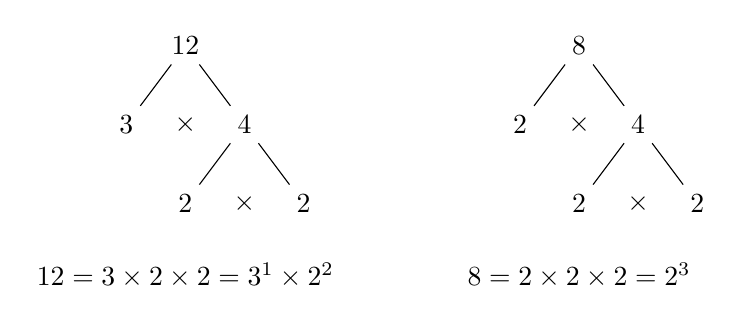
\begin{tikzpicture}[
  style={sibling distance=1.5cm, level distance=1cm},
]
  % First tree for 12
  \node (root) {$12$}
    child {node (a) {$3$}}
    child {node (b) {$4$}
      child {node (c) {$2$}}
      child {node (d) {$2$}}
    };
\path (a) -- node[midway] {$\times$} (b);
\path (c) -- node[midway] {$\times$} (d);
\node[below=.4cm of c] {$12 = 3 \times 2 \times 2 = 3^1\times 2^2$};

  % Second tree for 8
  \begin{scope}[xshift=5cm]
  \node (root2) {$8$}
    child {node (e) {$2$}}
    child {node (f) {$4$}
      child {node (g) {$2$}}
      child {node (h) {$2$}}
    };
\path (e) -- node[midway] {$\times$} (f);
\path (g) -- node[midway] {$\times$} (h);
\node[below=.4cm of g] {$8 = 2 \times 2 \times 2 = 2^3$};
  \end{scope}
\end{tikzpicture}
\end{center}
\end{itemize}

\begin{exercises}
\item
\label{Ex:factor_tree}
Fill in the missing numbers in the tree diagrams below.
\begin{center}
\begin{tikzpicture}[
    style={sibling distance=1.5cm, level distance=1cm}
]
  % First tree for 12
  \node (root) {$16$}
    child {node (a) {$\boxed{\phantom{2}}$}}
    child {node (b) {$8$}
      child {node (c) {$2$}}
      child {node (d) {$\boxed{\phantom{4}}$}
        child {node (e) {$2$}}
        child {node (f) {$2$}}
      }
    };
\path (a) -- node[midway] {$\times$} (b);
\path (c) -- node[midway] {$\times$} (d);
\path (e) -- node[midway] {$\times$} (f);
\node[below=.4cm of e] {$16 = \boxed{\phantom{2}} \times 2 \times 2 \times 2=2^{\boxed{\phantom{4}}}$};

  % Second tree for 20
  \begin{scope}[xshift=6cm]
  \node (root2) {$20$}
    child {node (e) {$2$}}
    child {node (f) {$\boxed{\phantom{10}}$}
      child {node (g) {$\boxed{\phantom{2}}$}}
      child {node (h) {$5$}}
    };
\path (e) -- node[midway] {$\times$} (f);
\path (g) -- node[midway] {$\times$} (h);
\node[below=.4cm of g] {$20 = 2 \times \boxed{\phantom{2}} \times 5=2^{\boxed{\phantom{2}}}\times 5^1$};
  \end{scope}
\end{tikzpicture}
\end{center}
\end{exercises}

\begin{itemize}
\item 
To build the \underbar{least common multiple}, multiply the prime factors that appear in each number. If a prime only occurs in one of the original numbers, use the original index. If a prime occurs in both original numbers, with a different index in each, use the larger index. For example,
\begin{itemize}
\item
Above we showed $12=3^1\times 2^2$ and $8=2^3$.
\item
The factor 2 occurs twice in 12, but three times in 8.
\item
So the least common multiple of 12 and 8 is $3^1\times 2^3 = 24$.
\end{itemize}
\end{itemize}

\begin{exercises}
\item 
In exercise \ref{Ex:factor_tree} we showed $16=2^{\boxed{\phantom{4}}}$ and $20=2^{\boxed{\phantom{2}}}\times 5^1$. So the least common multiple of 16 and 20 is $2^{\boxed{\phantom{4}}}\times5^1 = \boxed{\phantom{80}}.$
\item
Let's find the least common multiple of 18 and 24. First, draw factor trees for 18 and 24.
\begin{center}
\begin{tikzpicture}[
    style={sibling distance=1.5cm, level distance=1cm}
]
  % First tree for 18
  \node (root) {$18$}
    child {node (a) {$2$}}
    child {node (b) {$9$}
      child {node (c) {$\boxed{\phantom{3}}$}}
      child {node (d) {$\boxed{\phantom{3}}$}}
    };
\path (a) -- node[midway] {$\times$} (b);
\path (c) -- node[midway] {$\times$} (d);
\node[below=.4cm of c] {$18 = 2 \times \boxed{\phantom{3}} \times \boxed{\phantom{3}} = 2^1 \times \boxed{\phantom{3} }^{2}$};

  % Second tree for 24
  \begin{scope}[xshift=6cm]
  \node (root2) {$24$}
    child {node (e) {$3$}}
    child {node (f) {$\boxed{\phantom{8}}$}
      child {node (g) {$2$}}
      child {node (h) {$4$}
        child {node (i) {$\boxed{\phantom{2}}$}}
        child {node (j) {$\boxed{\phantom{2}}$}}
      }
    };
\path (e) -- node[midway] {$\times$} (f);
\path (g) -- node[midway] {$\times$} (h);
\path (i) -- node[midway] {$\times$} (j);
\node[below=.4cm of i] {$24 = 3\times2\times \boxed{\phantom{2}} \times \boxed{\phantom{2}} = 3^1 \times 2^{\boxed{\phantom{3}}}$};
  \end{scope}
\end{tikzpicture}
\end{center}
The factor 2 occurs once in 18 and \boxed{\phantom{3}} times in 24. The factor 3 occurs \boxed{\phantom{2}} times in 18 and once in 24. So the least common multiple of 18 and 24 is $2^{\boxed{\phantom{3}}}\times 3^{\boxed{\phantom{2}}} = \boxed{\phantom{72}}.$
\end{exercises}

\bibliographystyle{ametsocV6}
\bibliography{references}

\end{document}